\documentclass{ltjsbook}%
\usepackage{amssymb}%
\usepackage{amsthm}%
\usepackage{eulervm}%
\usepackage[%
  twoside,%
  paperwidth = 188mm,%
  paperheight = 263mm,%
  layoutwidth = 182mm,%
  layoutheight = 257mm,%
  layouthoffset = 3mm,%
  layoutvoffset = 3mm,%
  textwidth = 160mm,%
  textheight = 240mm,%
  left = 11mm,%
  right = 11mm,%
  top = 17mm,%
  bottom = 10mm,%
  headheight = 5mm,%
  headsep = 6mm%
]{geometry}%
\usepackage{luatexja-fontspec}%
\usepackage{mathtools}%
\usepackage{proof}%
\usepackage{tikz}%
\usepackage{titlesec}%
\usepackage{titletoc}%
\usepackage{xpatch}%
% amsthm
\renewcommand\proofname{証明}%
\newtheorem{theorem}{定理}[section]%
\newtheorem{lemma}{補題}[section]%
\newtheorem{definition}{定義}[section]%
\newtheorem{example}{例}[section]%
% luatexja-fontspec
\setmainfont{Novelty Light}%
\setsansfont{Novelty Light}%
\setmonofont{Journal}%
\setmainjfont{CandGReithic04}%
\setsansjfont{CandGReithic04}%
\newfontfamily\ebgaramond{EB Garamond}%
\newfontfamily\news{C4_news_R}%
\newjfontfamily\sbnreim{vsbmitaM}%
\newfontfamily\terra{Terra Narrow}%
% mathtools
\mathtoolsset{showonlyrefs = true}%
% tikz
\usetikzlibrary{arrows}%
\usetikzlibrary{lindenmayersystems}%
\pgfdeclarelindenmayersystem{Hilbert curve}{%
  \rule{L -> +RF-LFL-FR+}%
  \rule{R -> -LF+RFR+FL-}}%
% titlesec
\newpagestyle{techbookfest}{%
  \sethead[%
    {\ebgaramond\textit{\thepage}}][][]{}{}{%
    {\ebgaramond\textit{\thepage}}}%
  \setfoot[][][]{}{}{}}%
\assignpagestyle{\chapter}{techbookfest}%
\xpretocmd\chapter{\pagestyle{techbookfest}}{}{}%
\titleformat{\chapter}[block]{\Large\centering}{%
  \prechaptername\thechapter\postchaptername\quad}{0mm}{}%
\titleformat{\section}[block]{§\thesection.\quad}{}{0mm}{}%
% titletoc
\titlecontents{chapter}[5\zw]{%
  %\addvspace{1\zh}
  \contentslabel[{\thecontentslabel}]{5\zw}}{}{}{%
  \normalsize\hspace*{\fill}{\ebgaramond{\textit{\contentspage}}}}%
\titlecontents{section}[6\zw]{\contentslabel[%
    \S\thecontentslabel.]{6\zw}}{}{}{%
  \normalsize\titlerule*[1.5mm]{.}{\ebgaramond{\textit{\contentspage}}}}%
% personal commands
\newcommand\lemmaname{補題}%
\newcommand\term[2]{\textbf{#1}{(\textit{#2})}}%
\newlength\logowidth%
\settowidth\logowidth{\terra\Large An Introduction to Lambda Calculus}%
\begin{document}%
\pagestyle{empty}%
\begin{tikzpicture}[remember picture, overlay]%
  \node [%
    minimum width = 686.0086mm,%
    minimum height = 263.0043mm%
  ] at (current page.center) {%
    \begin{minipage}[t][263.0043mm]{686.0086mm}%
      \begin{flushright}%
        \begin{minipage}[t][263.0043mm]{263.0043mm}%
          \begin{tikzpicture}%
            \shadedraw%
              [bottom color=white, top color=white, draw=black, thick]%
              [l-system =%
                {Hilbert curve, axiom=L, order=7, step=2.0709mm, angle=90}]%
              lindenmayer system;%
          \end{tikzpicture}%
        \end{minipage}%
      \end{flushright}%
    \end{minipage}};%
\end{tikzpicture}%
\begin{tikzpicture}[remember picture, overlay]%
  \node [%
    minimum width = \paperwidth,%
    minimum height = \paperheight%
  ] at (current page.center) {%
    \begin{minipage}[t][\textheight]{\textwidth}%
      \vspace*{55.27864mm}%
      \hspace*{\the\dimexpr(\logowidth-0.25\textwidth)/2\relax}%
      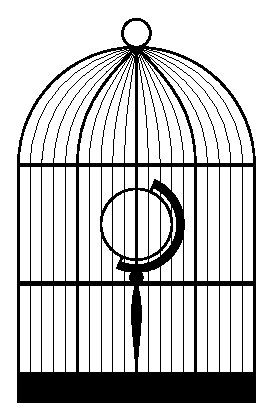
\includegraphics{logo.eps}%
    \end{minipage}};%
\end{tikzpicture}%
\begin{tikzpicture}[remember picture, overlay]%
  \node [%
    minimum width = \paperwidth,%
    minimum height = \paperheight%
  ] at (current page.center) {%
    \begin{minipage}[t][\textheight]{\textwidth}%
      \vspace*{0.5\textheight}%
      \begin{minipage}[t][0.125\textheight]{\textwidth}%
        \begin{minipage}[t][10mm]{\the\logowidth}%
          \vfill%
          {\terra\small\textit{Wir müssen wissen. Wir werden wissen.}}%
        \end{minipage}%
        \vfill%
        \begin{minipage}[t][15mm]{\the\logowidth}%
          \vspace*{\fill}%
          {\terra\Large An Introduction to Lambda Calculus}%
          {\news\scriptsize ラ\hspace*{\fill}ム\hspace*{\fill}ダ\hspace*{\fill}%
            計\hspace*{\fill}算\hspace*{\fill}入\hspace*{\fill}門}%
          \vspace*{\fill}%
        \end{minipage}%
        \vfill%
        \begin{minipage}[t][10mm]{\the\logowidth}%
          \hfill%
          {\sbnreim 川向薫}%
        \end{minipage}%
      \end{minipage}%
    \end{minipage}};%
\end{tikzpicture}%
\cleardoublepage%
\let\originalcleardoublepage\cleardoublepage%
\let\cleardoublepage\clearpage%
%\pagestyle{techbookfest}%
\frontmatter%
\chapter{はしがき}%
\hspace*{1\zw}本書はひとつのラムダ計算の入門書です.%
本書では型なしラムダ計算を扱います.%
\tableofcontents%
\mainmatter%
\chapter{型なしラムダ計算}%
\label{chap:untyped}%
\section{構文}%
\label{untyped:syntax}%
\begin{definition}%
  \par\term{変数}{variable}%
  \begin{equation}%
    \begin{array}{lrl}%
      \mathit{x}_1^{},\mathit{x}_2^{},\cdots%
      & \Coloneqq & x_1^{}\\%
      &         | & x_2^{}\\%
      &         | & \vdots%
    \end{array}%
  \end{equation}%
\end{definition}%
\begin{definition}%
\term{項}{term}%
\begin{equation}%
  \begin{array}{lrl}%
    \mathit{e}_1^{},\mathit{e}_2^{},\mathit{e}_3^{},\cdots%
    & \Coloneqq & \mathit{x}_1^{}\\%
    &         | & (\mathit{e}_1^{}\mathit{e}_2^{})\\%
    &         | & (\lambda\mathit{x}_2^{}\mathit{e}_3^{})%
  \end{array}%
\end{equation}%
\end{definition}%
\par$x_1^{}$や$x_2^{}$は(具体的な)変数ですが$\mathit{x}_1^{}$や$\mathit{x}_2^{}$は%
変数を表すメタ変数です.$\mathit{e}_1^{}$や$\mathit{e}_2^{}$は%
項を表すメタ変数です.メタ変数が出現する項をメタ項と呼びます.%
たとえば$(\lambda x_1^{}(\lambda x_2^{}x_1^{}))$は(具体的な)項ですが%
$(\lambda\mathit{x}_1^{}(\lambda\mathit{x}_2^{}\mathit{x}_1^{}))$はメタ項です.%
(具体的な)項を書くことはほとんどありませんので,%
メタ項を指して単に項と呼びますが,(具体的な)項を指しているわけではない%
ことに注意してください.このような区別をしばしば%
\term{メタ}{meta}レベルや\term{対象}{object}レベルと呼びます.%
\par$\mathit{e}_1^{}$の構造についての帰納法を%
$\mathit{e}_1^{}$の定義による帰納法と呼び,%
まず\term{基礎ケース}{base case}すなわち%
命題$P(\mathit{x}_1^{})$が成りたつことを%
証明し,\term{帰納ステップ}{induction step}すなわち%
$\mathit{e}_1^{},\mathit{e}_2^{},\mathit{e}_3^{}$について命題%
$P(\mathit{e}_1^{}),P(\mathit{e}_2^{}),P(\mathit{e}_3^{})$が成りたつ%
という仮定------\term{帰納法の仮定}{induction hypothesis}------のもとで命題%
$P(\mathit{e}_1^{}\mathit{e}_2^{}),P(\lambda\mathit{x}_2^{}\mathit{e}_3^{})$%
が成りたつことを証明します.それで命題%
$\forall\mathit{e}_4^{}P(\mathit{e}_4^{})$が証明されたことになります.%
再帰に似ていますが,CoqのFixpointのように%
``構造的に小さな''ものでしか帰納法の仮定は成立しません.%
\section{長さ}%
\label{sect:length}%
\begin{definition}%
項の\term{長さ}{length}%
\begin{equation}%
  length(\mathit{e}_1^{}) \coloneqq \begin{cases}%
    1 & \mathit{e}_1^{} = \mathit{x}_1^{}\\%
    length(\mathit{e}_2^{}) + length(\mathit{e}_3^{}) + 1%
    & \mathit{e}_1^{} = (\mathit{e}_2^{}\mathit{e}_3^{})\\%
    length(\mathit{e}_2^{}) + 1 & \mathit{e}_1^{} = (\lambda\mathit{x}\mathit{e}_2^{})%
  \end{cases}%
\end{equation}%
\end{definition}%
\par$length(\mathit{e}_1^{})=n$についての帰納法を$\mathit{e}_1^{}$の長さに関する%
帰納法と呼びます.長さに関する帰納法では,まず$length(\mathit{e}_1^{}) = 1$%
となるような$\mathit{e}_1^{}$すなわち$\mathit{x}_1^{}$について命題$P(\mathit{x}_1^{})$が%
成りたつことを証明し,$length(\mathit{e})\leqq k$となるような%
すべての$\mathit{e}$について命題$P(\mathit{e})$が成りたつと仮定した%
うえで$length(\mathit{e}_1^{}) = k + 1$となるような$\mathit{e}_1^{}$すなわち%
$(\mathit{e}_2^{}\mathit{e}_3^{}),(\lambda\mathit{x}_2^{}\mathit{e}_4^{})$%
について命題%
$P(\mathit{e}_2^{}\mathit{e}_3^{}),P(\lambda\mathit{x}_2^{}\mathit{e}_4^{})$%
が成りたつことを証明します.%
ここで$length(\mathit{e}_2^{})\leqq length(\mathit{e}_2^{}\mathit{e}_3^{})$%
かつ$length(\mathit{e}_3^{})\leqq length(\mathit{e}_2^{}\mathit{e}_3^{})$%
かつ$length(\mathit{e}_4^{})\leqq length(\lambda\mathit{x}_2^{}\mathit{e}_4^{})$なので%
$P(\mathit{e}_2^{}),P(\mathit{e}_3^{}),P(\mathit{e}_4^{})$が%
成りたつことは仮定してよいのです.%
$length(\mathit{e})\leqq k$であることさえ証明できれば%
仮定できるので,``構造的に小さくなくとも''%
再帰できる点で定義による帰納法とは異なります.%
\section{自由変数}%
\label{untyped:fv}%
\begin{definition}%
自由変数の集合%
\begin{equation}%
  FV(\mathit{e}_1^{}) \coloneqq \begin{cases}%
    \{\mathit{x}_1^{}\} & \mathit{e}_1^{} = \mathit{x}_1^{}\\%
    FV(\mathit{e}_2^{})\cup FV(\mathit{e}_3^{})%
    & \mathit{e}_1^{} = (\mathit{e}_2^{}\mathit{e}_3^{})\\%
    FV(\mathit{e}_2^{})\setminus\{\mathit{x}_1^{}\}%
    & \mathit{e}_1^{} = (\lambda\mathit{x}_1^{}\mathit{e}_2^{})%
  \end{cases}%
\end{equation}%
\end{definition}%
\section{束縛変数}%
\label{untyped:bv}%
\begin{definition}%
束縛変数の集合%
\begin{equation}%
  BV(\mathit{e}_1^{}) \coloneqq \begin{cases}%
    \emptyset & \mathit{e}_1^{} = \mathit{x}_1^{}\\%
    BV(\mathit{e}_2^{})\cup BV(\mathit{e}_3^{})%
    & \mathit{e}_1^{} = (\mathit{e}_2^{}\mathit{e}_3^{})\\%
    BV(\mathit{e}_2^{})\cup\{\mathit{x}_1^{}\}%
    & \mathit{e}_1^{} = (\lambda\mathit{x}_1^{}\mathit{e}_2^{})%
  \end{cases}%
\end{equation}%
\end{definition}%
\section{変数}%
\label{untyped:v}%
\begin{definition}%
変数の集合%
\begin{equation}%
  V(\mathit{e}_1^{}) \coloneqq FV(\mathit{e}_1^{})\cup BV(\mathit{e}_1^{})%
\end{equation}%
\end{definition}%
\section{代入}%
\label{untyped:subst}%
\begin{definition}%
\term{代入}{substitution}%
\begin{equation}%
  [\mathit{e}_1^{}/\mathit{x}_1^{}]\mathit{e}_2^{} \coloneqq \begin{cases}%
    \mathit{e}_1^{} & \mathit{e}_2^{} = \mathit{x}_2^{}\land\mathit{x}_1^{}=\mathit{x}_2^{}\\%
    \mathit{e}_2^{}%
    & \mathit{e}_2^{} = \mathit{x}_2^{}\land\mathit{x}_1^{}\neq\mathit{x}_2^{}\\%
    ([\mathit{e}_1^{}/\mathit{x}_1^{}]\mathit{e}_3^{}%
      [\mathit{e}_1^{}/\mathit{x}_1^{}]\mathit{e}_4^{})%
    & \mathit{e}_2^{} = (\mathit{e}_3^{}\mathit{e}_4^{})\\%
    \mathit{e}_2^{}%
    & \mathit{e}_2^{} = (\lambda\mathit{x}_2^{}\mathit{e}_3^{})%
    \land \mathit{x}_1^{} = \mathit{x}_2^{}\\%
    (\lambda\mathit{x}_3^{}[\mathit{e}_1^{}/\mathit{x}_1^{}][\mathit{x}_3^{}/\mathit{x}_2^{}]%
    \mathit{e}_3^{})%
    & \mathit{e}_2^{} = (\lambda\mathit{x}_2^{}\mathit{e}_3^{})%
    \land \mathit{x}_1^{} \neq \mathit{x}_2^{}%
    \land\mathit{x}_1^{}\neq\mathit{x}_3^{}%
    \land\mathit{x}_2^{}\neq\mathit{x}_3^{}%
    \land\mathit{x}_3^{}\not\in V(\mathit{e}_1^{})%
    \land\mathit{x}_3^{}\not\in V(\mathit{e}_2^{})%
  \end{cases}%
\end{equation}%
\end{definition}%
\begin{lemma}%
  \label{lemma:subst_len}%
  $\forall\mathit{x}_1^{}\forall\mathit{x}_2^{}\forall\mathit{e}_1^{}%
  (length([\mathit{x}_1^{}/\mathit{x}_2^{}]\mathit{e}_1^{})=length(\mathit{e}_1^{}))$.%
\end{lemma}%
\begin{proof}%
  $\mathit{x}_1^{},\mathit{x}_2^{},\mathit{e}_1^{}$を固定し,%
  $[\mathit{x}_1^{}/\mathit{x}_2^{}]\mathit{e}_1^{}$の定義による帰納法で%
  証明する.%
  \begin{itemize}%
  \item $[\mathit{x}_1^{}/\mathit{x}_2^{}]\mathit{e}_1^{} = \mathit{x}_1^{}$の場合.%
    $\mathit{e}_1^{} = \mathit{x}_2^{}$なので,%
    \begin{align}%
      length([\mathit{x}_1^{}/\mathit{x}_2^{}]\mathit{e}_1^{})&=length(\mathit{x}_1^{})\\%
      &=1\\%
      &=length(\mathit{x}_2^{})\\%
      &=length(\mathit{e}_1^{})%
    \end{align}%
  \item $[\mathit{x}_1^{}/\mathit{x}_2^{}]\mathit{e}_1^{} = \mathit{e}_1^{}$の場合.%
    明らかに%
    $length([\mathit{x}_1^{}/\mathit{x}_2^{}]\mathit{e}_1^{})=length(\mathit{e}_1^{})$.%
  \item $[\mathit{x}_1^{}/\mathit{x}_2^{}]\mathit{e}_1^{}%
    = ([\mathit{x}_1^{}/\mathit{x}_2^{}]\mathit{e}_2^{}[\mathit{x}_1^{}/\mathit{x}_2^{}]\mathit{e}_3^{})$の場合.%
    帰納法の仮定:%
    \begin{align}%
    length([\mathit{x}_1^{}/\mathit{x}_2^{}]\mathit{e}_2^{})&=length(\mathit{e}_2^{})\\%
    length([\mathit{x}_1^{}/\mathit{x}_2^{}]\mathit{e}_3^{})&=length(\mathit{e}_3^{})%
    \end{align}%
    したがって,%
    \begin{align}%
    length([\mathit{x}_1^{}/\mathit{x}_2^{}]\mathit{e}_1^{})%
    &=length([\mathit{x}_1^{}/\mathit{x}_2^{}]\mathit{e}_2^{}%
    [\mathit{x}_1^{}/\mathit{x}_2^{}]\mathit{e}_3^{})\\%
    &=length([\mathit{x}_1^{}/\mathit{x}_2^{}]\mathit{e}_2^{})%
    +length([\mathit{x}_1^{}/\mathit{x}_2^{}]\mathit{e}_3^{})+1\\%
    &=length(\mathit{e}_2^{})+length(\mathit{e}_3^{})+1\\%
    &=length(\mathit{e}_2^{}\mathit{e}_3^{})\\%
    &=length(\mathit{e}_1^{})%
    \end{align}%
  \item $[\mathit{x}_1^{}/\mathit{x}_2^{}]\mathit{e}_1^{}%
    = (\lambda\mathit{x}_4^{}[\mathit{x}_1^{}/\mathit{x}_2^{}]%
    [\mathit{x}_4^{}/\mathit{x}_3^{}]\mathit{e}_2^{})$の場合.%
    帰納法の仮定:%
    \begin{align}%
      length([\mathit{x}_1^{}/\mathit{x}_2^{}][\mathit{x}_4^{}/\mathit{x}_3^{}]\mathit{e}_2^{})%
      &=length([\mathit{x}_4^{}/\mathit{x}_3^{}]\mathit{e}_2^{})\\%
      length([\mathit{x}_4^{}/\mathit{x}_3^{}]\mathit{e}_2^{})%
      &=length(\mathit{e}_2^{})%
    \end{align}%
    したがって,$\mathit{e}_1^{}=(\lambda\mathit{x}_3^{}\mathit{e}_2^{})$なので,%
    \begin{align}%
    length([\mathit{x}_1^{}/\mathit{x}_2^{}]\mathit{e}_1^{})%
    &=length(\lambda\mathit{x}_4^{}[\mathit{x}_1^{}/\mathit{x}_2^{}][\mathit{x}_4^{}/\mathit{x}_3^{}]\mathit{e}_2^{})\\%
    &=length([\mathit{x}_1^{}/\mathit{x}_2^{}][\mathit{x}_4^{}/\mathit{x}_3^{}]\mathit{e}_2^{})+1\\%
    &=length([\mathit{x}_4^{}/\mathit{x}_3^{}]\mathit{e}_2^{})+1\\%
    &=length(\mathit{e}_2^{})+1\\%
    &=length(\lambda\mathit{x}_3^{}\mathit{e}_2^{})\\%
    &=length(\mathit{e}_1^{})%
    \end{align}%
  \end{itemize}%
\end{proof}%
\begin{lemma}%
  \label{lemma:subst_trans}%
  $\forall\mathit{x}_1^{}\forall\mathit{x}_2^{}\forall\mathit{x}_3^{}\forall\mathit{e}_1^{}%
  ([\mathit{x}_1^{}/\mathit{x}_2^{}][\mathit{x}_2^{}/\mathit{x}_3^{}]\mathit{e}_1^{}%
  =[\mathit{x}_1^{}/\mathit{x}_3^{}]\mathit{e}_1^{})$.%
\end{lemma}%
\begin{proof}%
  証明は簡単.%
\end{proof}%
\section{$\alpha$-変換}%
\label{sect:alpha}%
\begin{definition}%
\term{$\alpha$-同値}{$\alpha$-congruence}%
\begin{equation}%
  \mathit{e}_1^{}\equiv\mathit{e}_2^{} \coloneqq \begin{cases}%
    \mathit{x}_1^{} = \mathit{x}_2^{}%
    & \mathit{e}_1^{} = \mathit{x}_1^{}%
    \land \mathit{e}_2^{} = \mathit{x}_2^{}\\%
    \mathit{e}_3^{}\equiv\mathit{e}_5^{}\land\mathit{e}_4^{}\equiv\mathit{e}_6^{}%
    & \mathit{e}_1^{} = (\mathit{e}_3^{}\mathit{e}_4^{})%
    \land \mathit{e}_2^{} = (\mathit{e}_5^{}\mathit{e}_6^{})\\%
    {}[\mathit{x}_3^{}/\mathit{x}_1^{}]\mathit{e}_3^{}%
    \equiv{}[\mathit{x}_3^{}/\mathit{x}_2^{}]\mathit{e}_4^{}%
    & \mathit{e}_1^{} = (\lambda\mathit{x}_1^{}\mathit{e}_3^{})%
    \land \mathit{e}_2^{} = (\lambda\mathit{x}_2^{}\mathit{e}_4^{})%
    \land \mathit{x}_3^{}\not\in V(\mathit{e}_1^{})%
    \land \mathit{x}_3^{}\not\in V(\mathit{e}_2^{})%
  \end{cases}%
\end{equation}%
\end{definition}%
\par$\mathit{e}_1^{}\equiv\mathit{e}_2^{}$が定義されないことを単に%
$\mathit{e}_1^{}\not\equiv\mathit{e}_2^{}$と書きます.%
$\mathit{e}_1^{}\equiv\mathit{e}_2^{}$は簡単には%
変数名の違いを無視した同値関係です.たとえば%
$(\lambda x_1^{}x_1^{})\neq(\lambda x_2^{}x_2^{})$ですが%
$(\lambda x_1^{}x_1^{})\equiv(\lambda x_2^{}x_2^{})$です.%
\begin{lemma}%
  \label{lemma:alpha_len}%
  $\forall\mathit{e}_1^{}\forall\mathit{e}_2^{}%
  (\mathit{e}_1^{}\equiv\mathit{e}_2^{}\rightarrow%
  length(\mathit{e}_1^{})=length(\mathit{e}_2^{}))$.%
\end{lemma}%
\begin{proof}%
  証明は簡単.%
\end{proof}%
簡単のため$\mathit{e}_1^{}\equiv\mathit{e}_2^{}$のとき,%
$\mathit{e}_1^{},\mathit{e}_2^{}$両方の長さに関する帰納法で証明することがあります.%
2重帰納法ではありませんので注意してください.%
帰納法は基本的にひとつの自然数や構造に対してしかできませんが,%
項の\term{n-組}{n-tuple}$(\mathit{e}_1^{},\cdots,\mathit{e}_n^{})$というひとつの%
構造を考えれば,%
$\mathit{e}_1^{}\equiv\mathit{e}_2^{}かつ\cdots%
かつ\mathit{e}_{n-1}^{}\equiv\mathit{e}_n^{}$%
という前提なら%
$length(\mathit{e}_1^{})=\cdots=length(\mathit{e}_n^{})$ですから,%
\begin{equation}%
  length_n^{}(\mathit{e}_1^{},\cdots,\mathit{e}_n^{})\coloneqq%
  length(\mathit{e}_1^{})%
\end{equation}%
を与えれば,項のn-組の長さに関する帰納法ができます.%
\begin{lemma}%
  \label{lemma:alpha_fequal}%
  $\forall\mathit{f}\forall\mathit{e}_1^{}\forall\mathit{e}_2^{}%
  (\mathit{e}_1^{}\equiv\mathit{e}_2^{}\rightarrow%
  \mathit{f}(\mathit{e}_1^{})\equiv\mathit{f}(\mathit{e}_2^{}))$.%
\end{lemma}%
\begin{proof}%
  証明は簡単.%
\end{proof}%
\begin{lemma}%
  $\alpha$-同値は反射的である.すなわち,%
  $\forall\mathit{e}_1^{}(\mathit{e}_1^{}\equiv\mathit{e}_1^{})$.%
\end{lemma}%
\begin{proof}%
  $\mathit{e}_1^{}$を固定し,$\mathit{e}_1^{}$の長さに関する帰納法で証明する.%
  \begin{itemize}%
  \item $length(\mathit{e}_1^{})=1$の場合.%
  \begin{itemize}%
  \item $\mathit{e}_1^{}=\mathit{x}_1^{}$の場合.$\mathit{x}_1^{}=\mathit{x}_1^{}$なので,%
    $\alpha$-同値の定義により$\mathit{e}_1^{}\equiv\mathit{e}_1^{}$である.%
  \end{itemize}%
  \item $length(\mathit{e}_1^{})=k + 1$の場合.%
  \begin{itemize}%
  \item $\mathit{e}_1^{}=(\mathit{e}_2^{}\mathit{e}_3^{})$の場合.帰納法の仮定:%
    \begin{align}%
      \mathit{e}_2^{}&\equiv \mathit{e}_2^{}\\%
      \mathit{e}_3^{}&\equiv \mathit{e}_3^{}%
    \end{align}%
    したがって$\mathit{e}_2^{}\equiv \mathit{e}_2^{}%
    \land \mathit{e}_3^{}\equiv \mathit{e}_3^{}$なので,%
    $\alpha$-同値の定義により$\mathit{e}_1^{}\equiv \mathit{e}_1^{}$%
    である.%
  \item $\mathit{e}_1^{}=(\lambda \mathit{x}_1^{}\mathit{e}_2^{})$の場合.%
    帰納法の仮定:%
    \begin{align}%
      \mathit{e}_2^{}\equiv\mathit{e}_2^{}%
    \end{align}%
    また\lemmaname\ref{lemma:subst_len}により帰納法の仮定は%
    $[\mathit{x}_2^{}/\mathit{x}_1^{}]\mathit{e}_2^{}\equiv%
    [\mathit{x}_2^{}/\mathit{x}_1^{}]\mathit{e}_2^{}$と変形できるから,%
    $\alpha$-同値の定義により$\mathit{e}_1^{}\equiv \mathit{e}_1^{}$である.%
  \end{itemize}%
  \end{itemize}%
\end{proof}%
\begin{lemma}%
  $\alpha$-同値は対称的である.すなわち,%
  $\forall\mathit{e}_1^{}\forall\mathit{e}_2^{}%
  (\mathit{e}_1^{}\equiv \mathit{e}_2^{}\rightarrow\mathit{e}_2^{}\equiv \mathit{e}_1^{})$.%
\end{lemma}%
\begin{proof}%
  $\mathit{e}_1^{},\mathit{e}_2^{}$を固定し,%
  $\mathit{e}_1^{},\mathit{e}_2^{}$の長さに関する帰納法で証明する.前提:%
  \begin{align}%
    \mathit{e}_1^{}\equiv \mathit{e}_2^{}%
  \end{align}%
  \begin{itemize}%
  \item $length(\mathit{e}_1^{})=length(\mathit{e}_2^{})=1$の場合.%
  \begin{itemize}%
  \item $\mathit{e}_1^{}=\mathit{x}_1^{},\mathit{e}_2^{}=\mathit{x}_2^{}$の場合.%
    前提を計算すれば$\mathit{x}_1^{}=\mathit{x}_2^{}$となるので,%
    $\mathit{x}_2^{}=\mathit{x}_1^{}$.したがって%
    $\alpha$-同値の定義により$\mathit{e}_2^{}\equiv \mathit{e}_1^{}$である.%
  \end{itemize}%
  \item $length(\mathit{e}_1^{})=length(\mathit{e}_2^{})=k+1$の場合.%
  \begin{itemize}%
  \item $\mathit{e}_1^{}=(\mathit{e}_3^{}\mathit{e}_4^{}),%
    \mathit{e}_2^{}=(\mathit{e}_5^{}\mathit{e}_6^{})$の場合.帰納法の仮定:%
    \begin{align}%
    \mathit{e}_3^{}\equiv\mathit{e}_5^{}\rightarrow%
    \mathit{e}_5^{}\equiv\mathit{e}_3^{}\\%
    \mathit{e}_4^{}\equiv\mathit{e}_6^{}\rightarrow%
    \mathit{e}_6^{}\equiv\mathit{e}_4^{}%
    \end{align}%
    また前提を計算すれば%
    $\mathit{e}_3^{}\equiv\mathit{e}_5^{}\land\mathit{e}_4^{}\equiv\mathit{e}_6^{}$となるので,%
    $\mathit{e}_5^{}\equiv\mathit{e}_3^{}\land\mathit{e}_6^{}\equiv\mathit{e}_4^{}$であり,%
    $\alpha$-同値の定義により$\mathit{e}_2^{}\equiv \mathit{e}_1^{}$である.%
  \item $\mathit{e}_1^{}=(\lambda \mathit{x}_1^{}\mathit{e}_3^{}),%
    \mathit{e}_2^{}=(\lambda \mathit{x}_2^{}\mathit{e}_4^{})$の場合.帰納法の仮定:%
    \begin{align}%
    \mathit{e}_3^{}\equiv\mathit{e}_4^{}\rightarrow%
    \mathit{e}_4^{}\equiv\mathit{e}_3^{}%
    \end{align}%
    また前提を計算すれば${}[\mathit{x}_3^{}/\mathit{x}_1^{}]\mathit{e}_3^{}%
    \equiv{}[\mathit{x}_3^{}/\mathit{x}_2^{}]\mathit{e}_4^{}$となり,%
    \lemmaname\ref{lemma:subst_len}により帰納法の仮定は%
    \begin{align}%
    {}[\mathit{x}_3^{}/\mathit{x}_1^{}]\mathit{e}_3^{}%
    \equiv{}[\mathit{x}_3^{}/\mathit{x}_2^{}]\mathit{e}_4^{}\rightarrow%
    {}[\mathit{x}_3^{}/\mathit{x}_2^{}]\mathit{e}_4^{}%
    \equiv{}[\mathit{x}_3^{}/\mathit{x}_1^{}]\mathit{e}_3^{}%
    \end{align}%
    と変形できるから,${}[\mathit{x}_3^{}/\mathit{x}_2^{}]\mathit{e}_4^{}%
    \equiv{}[\mathit{x}_3^{}/\mathit{x}_1^{}]\mathit{e}_3^{}$である.したがって%
    $\alpha$-同値の定義により$\mathit{e}_2^{}\equiv \mathit{e}_1^{}$である.%
  \end{itemize}%
  \item $length(\mathit{e}_1^{})\neq length(\mathit{e}_2^{})$の場合.%
    前提と\lemmaname\ref{lemma:alpha_len}が矛盾するので,%
    このような場合は起こりえない.%
  \end{itemize}%
\end{proof}%
今回は最後の$length(\mathit{e}_1^{})\neq length(\mathit{e}_2^{})$の場合を%
明示しましたが,今後は省略します.%
\begin{lemma}%
  $\alpha$-同値は推移的である.すなわち,%
  $\forall\mathit{e}_1^{}\forall\mathit{e}_2^{}\forall\mathit{e}_3^{}%
  (\mathit{e}_1^{}\equiv \mathit{e}_2^{}\rightarrow\mathit{e}_2^{}\equiv \mathit{e}_3^{}%
  \rightarrow\mathit{e}_1^{}\equiv \mathit{e}_3^{})$.%
\end{lemma}%
\begin{proof}%
  $\mathit{e}_1^{},\mathit{e}_2^{},\mathit{e}_3^{}$を固定し,%
  $\mathit{e}_1^{},\mathit{e}_2^{},\mathit{e}_3^{}$の長さに関する帰納法で証明する.前提:%
  \begin{align}%
    \mathit{e}_1^{}&\equiv \mathit{e}_2^{}\\%
    \mathit{e}_2^{}&\equiv \mathit{e}_3^{}%
  \end{align}%
  \begin{itemize}%
  \item $length(\mathit{e}_1^{})=length(\mathit{e}_2^{})=length(\mathit{e}_3^{})=1$の%
    場合.%
  \begin{itemize}%
  \item $\mathit{e}_1^{}=\mathit{x}_1^{},\mathit{e}_2^{}=\mathit{x}_2^{},%
    \mathit{e}_3^{}=\mathit{x}_3^{}$の場合.%
    前提を計算すれば$\mathit{x}_1^{}=\mathit{x}_2^{}$かつ%
    $\mathit{x}_2^{}=\mathit{x}_3^{}$となる.したがって$\mathit{x}_1^{}=\mathit{x}_3^{}$%
    なので,$\alpha$-同値の定義により$\mathit{e}_1^{}\equiv \mathit{e}_3^{}$である.%
  \end{itemize}%
  \item $length(\mathit{e}_1^{})=length(\mathit{e}_2^{})=length(\mathit{e}_3^{})=k+1$%
  の場合.%
  \begin{itemize}%
  \item $\mathit{e}_1^{}=(\mathit{e}_4^{}\mathit{e}_5^{}),%
    \mathit{e}_2^{}=(\mathit{e}_6^{}\mathit{e}_7^{}),%
    \mathit{e}_3^{}=(\mathit{e}_8^{}\mathit{e}_9^{})$の場合.帰納法の仮定:%
    \begin{align}%
    \mathit{e}_4^{}\equiv\mathit{e}_6^{}\rightarrow%
    \mathit{e}_6^{}\equiv\mathit{e}_8^{}\rightarrow%
    \mathit{e}_4^{}\equiv\mathit{e}_8^{}\\%
    \mathit{e}_5^{}\equiv\mathit{e}_7^{}\rightarrow%
    \mathit{e}_7^{}\equiv\mathit{e}_9^{}\rightarrow%
    \mathit{e}_5^{}\equiv\mathit{e}_9^{}%
    \end{align}%
    また前提を計算すれば%
    $\mathit{e}_4^{}\equiv\mathit{e}_6^{}\land\mathit{e}_5^{}\equiv\mathit{e}_7^{}$かつ%
    $\mathit{e}_6^{}\equiv\mathit{e}_8^{}\land\mathit{e}_7^{}\equiv\mathit{e}_9^{}$と%
    なるので,%
    $\mathit{e}_4^{}\equiv\mathit{e}_8^{}\land\mathit{e}_5^{}\equiv\mathit{e}_9^{}$であり,%
    $\alpha$-同値の定義により$\mathit{e}_1^{}\equiv \mathit{e}_3^{}$である.%
  \item $\mathit{e}_1^{}=(\lambda \mathit{x}_1^{}\mathit{e}_4^{}),%
    \mathit{e}_2^{}=(\lambda \mathit{x}_2^{}\mathit{e}_5^{}),%
    \mathit{e}_3^{}=(\lambda \mathit{x}_3^{}\mathit{e}_6^{})$の場合.帰納法の仮定:%
    \begin{align}%
    \mathit{e}_4^{}\equiv\mathit{e}_5^{}\rightarrow%
    \mathit{e}_5^{}\equiv\mathit{e}_6^{}\rightarrow%
    \mathit{e}_4^{}\equiv\mathit{e}_6^{}%
    \end{align}%
    また前提を計算すれば%
    ${}[\mathit{x}_4^{}/\mathit{x}_1^{}]\mathit{e}_4^{}%
    \equiv{}[\mathit{x}_4^{}/\mathit{x}_2^{}]\mathit{e}_5^{}$かつ%
    ${}[\mathit{x}_5^{}/\mathit{x}_2^{}]\mathit{e}_5^{}%
    \equiv{}[\mathit{x}_5^{}/\mathit{x}_3^{}]\mathit{e}_6^{}$となり,%
    \lemmaname\ref{lemma:alpha_fequal}により%
    ${}[\mathit{x}_6^{}/\mathit{x}_4^{}]{}[\mathit{x}_4^{}/\mathit{x}_1^{}]\mathit{e}_4^{}%
    \equiv{}[\mathit{x}_6^{}/\mathit{x}_4^{}][\mathit{x}_4^{}/\mathit{x}_2^{}]\mathit{e}_5^{}$%
    かつ%
    ${}[\mathit{x}_6^{}/\mathit{x}_5^{}]{}[\mathit{x}_5^{}/\mathit{x}_2^{}]\mathit{e}_5^{}%
    \equiv{}[\mathit{x}_6^{}/\mathit{x}_5^{}][\mathit{x}_5^{}/\mathit{x}_3^{}]\mathit{e}_6^{}$%
    すなわち\lemmaname\ref{lemma:subst_trans}により%
    ${}[\mathit{x}_6^{}/\mathit{x}_1^{}]\mathit{e}_4^{}%
    \equiv{}[\mathit{x}_6^{}/\mathit{x}_2^{}]\mathit{e}_5^{}$かつ%
    ${}[\mathit{x}_6^{}/\mathit{x}_2^{}]\mathit{e}_5^{}%
    \equiv{}[\mathit{x}_6^{}/\mathit{x}_3^{}]\mathit{e}_6^{}$である.%
    \lemmaname\ref{lemma:subst_len}によりにより帰納法の仮定は%
    \begin{align}%
    {}[\mathit{x}_6^{}/\mathit{x}_1^{}]\mathit{e}_4^{}%
    \equiv{}[\mathit{x}_6^{}/\mathit{x}_2^{}]\mathit{e}_5^{}%
    \rightarrow%
    {}[\mathit{x}_6^{}/\mathit{x}_2^{}]\mathit{e}_5^{}%
    \equiv{}[\mathit{x}_6^{}/\mathit{x}_3^{}]\mathit{e}_6^{}%
    \rightarrow%
    {}[\mathit{x}_6^{}/\mathit{x}_1^{}]\mathit{e}_4^{}%
    \equiv{}[\mathit{x}_6^{}/\mathit{x}_3^{}]\mathit{e}_6^{}%
    \end{align}%
    と変形できるから,%
    ${}[\mathit{x}_6^{}/\mathit{x}_1^{}]\mathit{e}_4^{}%
    \equiv{}[\mathit{x}_6^{}/\mathit{x}_3^{}]\mathit{e}_6^{}$である.%
    ゆえに$\alpha$-同値の定義により$\mathit{e}_1^{}\equiv \mathit{e}_3^{}$である.%
  \end{itemize}%
  \end{itemize}%
\end{proof}%
\par$\mathit{e}_1^{}\equiv\mathit{e}_2^{}$のとき,%
$\mathit{e}_1^{}$を$\mathit{e}_2^{}$で置きかえることを%
\term{$\alpha$-変換}{$\alpha$-conversion}と呼びます.%
以後,$\mathit{e}_1^{}\equiv\mathit{e}_2^{}$は通常の等号と同様に,%
すなわち$\mathit{e}_1^{}\equiv\mathit{e}_2^{}$のときはいつでも%
$\mathit{e}_1^{}$を$\mathit{e}_2^{}$で置きかえてもよいと考えます.%
\section{$\beta$-変形}%
\label{sect:beta}%
\begin{definition}%
  \term{式}{expression}%
  \par$\mathit{e}_1^{},\mathit{e}_2^{}$が項ならば$\mathit{e}_1^{}\triangleright_1^{}\mathit{e}_2^{}$%
  と$\mathit{e}_1^{}\triangleright\mathit{e}_2^{}$を$\beta$-変形の\term{式}{expression}と呼ぶ.%
\end{definition}%
\begin{definition}%
1ステップの\term{$\beta$-変形}{$\beta$-reduction}%
\begin{equation}%
  \infer{%
    ((\lambda\mathit{x}_1^{}\mathit{e}_1^{})\mathit{e}_2^{})\triangleright_1^{}%
    [\mathit{e}_1^{}/\mathit{x}_1^{}]\mathit{e}_2^{}%
  }{%
  }%
\end{equation}%
\begin{equation}%
  \infer{%
    (\mathit{e}_1^{}\mathit{e}_3^{})\triangleright_1^{}(\mathit{e}_2^{}\mathit{e}_3^{})%
  }{%
    \mathit{e}_1^{}\triangleright_1^{}\mathit{e}_2^{}%
  }%
\end{equation}%
\begin{equation}%
  \infer{%
    (\mathit{e}_3^{}\mathit{e}_1^{})\triangleright_1^{}(\mathit{e}_3^{}\mathit{e}_2^{})%
  }{%
    \mathit{e}_1^{}\triangleright_1^{}\mathit{e}_2^{}%
  }%
\end{equation}%
\begin{equation}%
  \infer{%
    (\lambda\mathit{x}_1^{}\mathit{e}_1^{})\triangleright_1^{}%
    (\lambda\mathit{x}_1^{}\mathit{e}_2^{})%
  }{%
    \mathit{e}_1^{}\triangleright_1^{}\mathit{e}_2^{}%
  }%
\end{equation}%
\end{definition}%
\begin{definition}%
nステップの$\beta$-変形%
\begin{equation}%
  \infer{%
    \mathit{e}_1^{}\triangleright\mathit{e}_1^{}%
  }{%
  }%
\end{equation}%
\begin{equation}%
  \infer{%
    \mathit{e}_1^{}\triangleright\mathit{e}_3^{}%
  }{%
    \mathit{e}_1^{}\triangleright_1^{}\mathit{e}_2^{}%
  &%
    \mathit{e}_2^{}\triangleright\mathit{e}_3^{}%
  }%
\end{equation}%
\end{definition}%
\par 横線より上の部分を\term{前提}{premise},下の部分を\term{結論}{conclusion}%
と呼びます.推論規則をいくつか組みあわせた図を\term{推論図}{deduction}と%
呼びます.%
\begin{definition}%
\term{推論図}{deduction}%
\begin{itemize}%
\item 式$A$は推論図である.この形の推論図を\term{仮定}{assumption}と呼び,%
  前提は$\{A\}$で結論は$A$である.%
\item $\Pi_1^{},\cdots,\Pi_n^{}$を推論図とし,それぞれの結論を$A_1^{},\cdots,A_n^{}$と%
  する.$A_1^{},\cdots,A_n^{}$を前提とする推論規則が存在し,その結論が$B$ならば,%
  \begin{equation}%
    \infer{B}{\Pi_1^{}&\cdots&\Pi_n^{}}%
  \end{equation}%
  は推論図である.この形の推論図の前提は%
  $\Pi_1^{}の前提\cup\cdots\cup\Pi_n^{}の前提$であり,%
  結論は$B$である.%
\end{itemize}%
\end{definition}%
推論図の概念は,帰納的に定義するより例示したほうがわかりやすいかもしれません.%
つぎの推論図は,$(((\lambda x_1^{}(\lambda x_2^{} x_1^{}))x_3^{})x_4^{})$という項が%
nステップの$\beta$-変形で$x_3^{}$になるということを表しています.%
読みやすくするために代入はあらかじめ等価な項で置きかえてありますが,%
厳密には代入が出現する場所もあることに注意してください.%
\begin{example}%
  \begin{equation}%
    \infer{%
      (((\lambda x_1^{}(\lambda x_2^{} x_1^{}))x_3^{})x_4^{})\triangleright x_3^{}%
    }{%
      \infer{%
        (((\lambda x_1^{}(\lambda x_2^{} x_1^{}))x_3^{})x_4^{})\triangleright_1^{}%
        ((\lambda x_2^{} x_3^{})x_4^{})%
      }{%
        \infer{%
          ((\lambda x_1^{}(\lambda x_2^{} x_1^{}))x_3^{})\triangleright_1^{}%
          (\lambda x_2^{} x_3^{})%
        }{%
        }%
      }%
    &%
      \infer{%
        ((\lambda x_2^{} x_3^{})x_4^{})\triangleright x_3^{}%
      }{%
        \infer{%
          ((\lambda x_2^{} x_3^{})x_4^{})\triangleright_1^{}x_3^{}%
        }{%
        }%
      &%
        \infer{%
          x_3^{}\triangleright x_3^{}%
        }{%
        }%
      }%
    }%
  \end{equation}%
\end{example}%
\par このように1ステップの$\beta$-変形とnステップの$\beta$-変形を別々に定義する%
意味論をSmall Step Semanticsと呼びます.Small Step Semanticsの関心は%
1ステップの$\beta$-変形にありますので,nステップの$\beta$-変形を定義しないこと%
もあります.1ステップの$\beta$-変形を定義せず,%
いきなりnステップの$\beta$-変形を定義する意味論をBig Step Semanticsと呼びます.%
Big Step Semanticsでは$\Downarrow$という記号をもちいることが一般的です.%
Big Step Semanticsのほうがより実際の実装に近い意味論なのでプログラム言語の%
形式化ではよくもちいられますが,理論的な計算模型を考える場合には%
Small Step Semanticsがよくもちいられます.%
\par$\Pi$の前提が$\{A_1^{},\cdots,A_n^{}\}$で結論が$B$のとき,%
$\Pi$を$B$に至る推論図と呼び,%
$\Gamma=A_1^{},\cdots,A_n^{},A_{n+1}^{},\cdots,A_{n+m}^{}$を$\Pi$の仮定と呼びます.%
仮定は集合と同様に,順序や重複は気にしませんし,%
前提にない式が仮定に含まれていてもかまいません.%
さらに$\Gamma\vdash B$と書き,仮定$\Gamma$から$B$がでると読みます.%
とくに$n=0$かつ$m=0$すなわち$\Pi$の仮定が空のとき$\Pi$を証明図と呼び,%
$B$は\term{証明可能}{provable}であるといいます.%
$\mathit{e}_1^{}\triangleright_1^{}\mathit{e}_2^{}$が証明できるような%
$\mathit{e}_2^{}$が存在しないとき,$\mathit{e}_1^{}$は%
\term{$\beta$-正規形}{$\beta$-redux}であるといいます.%
$\mathit{e}_1^{}\triangleright\mathit{e}_2^{}$が証明でき,%
かつ$\mathit{e}_2^{}$が正規形であるとき,%
$\mathit{e}_1^{}$は正規形をもつといいます.%
正規形をもたない項が存在することに注意してください.%
たとえば,$((\lambda x_0x_0)(\lambda x_0x_0))$は正規形をもちません.%
\begin{definition}%
推論図の\term{長さ}{length}%
\begin{equation}%
  length(\Pi)\Coloneqq\begin{cases}%
  1&\Pi=A\\%
  length(\Pi_1^{})+\cdots+length(\Pi_n^{})+1%
  &\Pi=\begin{array}{c}\infer{A}{\Pi_1^{}&\cdots&\Pi_n^{}}\end{array}%
  \end{cases}%
\end{equation}%
\end{definition}%
\begin{lemma}%
  \label{lemma:beta_reduct1n}%
  $(\vdash\mathit{e}_1^{}\triangleright_1^{}\mathit{e}_2^{})\rightarrow%
  (\vdash\mathit{e}_1^{}\triangleright\mathit{e}_2^{})$.%
\end{lemma}%
\begin{proof}%
  \begin{equation}%
    \infer{%
      \mathit{e}_1^{}\triangleright\mathit{e}_2^{}%
    }{%
      \infer{\mathit{e}_1^{}\triangleright_1^{}\mathit{e}_2^{}}{}%
    &%
      \infer{\mathit{e}_2^{}\triangleright\mathit{e}_2^{}}{}%
    }%
  \end{equation}%
\end{proof}%
\begin{lemma}%
  \label{lemma:beta_reduct_trans}%
  nステップの$\beta$-変形は推移的である.すなわち,%
  $(\vdash\mathit{e}_1^{}\triangleright\mathit{e}_2^{})\rightarrow%
  (\vdash\mathit{e}_2^{}\triangleright\mathit{e}_3^{})\rightarrow%
  (\vdash\mathit{e}_1^{}\triangleright\mathit{e}_3^{})$.%
\end{lemma}%
\begin{proof}%
  $\mathit{e}_1^{}\triangleright\mathit{e}_2^{}$に至る証明図を$\Pi$とし,%
  $\Pi$の長さに関する帰納法で証明する.%
  \begin{itemize}%
  \item $length(\Pi)=1$ の場合.%
    $\mathit{e}_1^{}\triangleright\mathit{e}_3^{}$に至る証明図は%
    \begin{equation}%
      \infer{%
        \mathit{e}_1^{}\triangleright\mathit{e}_3^{}%
      }{%
        \infer{\mathit{e}_1^{}\triangleright\mathit{e}_1^{}}{}%
      &%
        \infer{\mathit{e}_1^{}\triangleright\mathit{e}_3^{}}{\Pi_1^{}&\cdots&\Pi_n^{}}%
      }%
    \end{equation}%
    という形をしているから,$\Pi$はいわば``むだな''証明図なので,%
    単にはぶけば%
    \begin{equation}%
      \infer{\mathit{e}_1^{}\triangleright\mathit{e}_3^{}}{\Pi_1^{}&\cdots&\Pi_n^{}}%
    \end{equation}%
    と変形できるからよい.%
  \item $length(\Pi)=k + 1$ の場合.%
    $\mathit{e}_1^{}\triangleright\mathit{e}_3^{}$に至る証明図は%
    \begin{equation}%
      \infer{%
        \mathit{e}_1^{}\triangleright\mathit{e}_3^{}%
      }{%
        \infer{%
          \mathit{e}_1^{}\triangleright\mathit{e}_2^{}%
        }{%
          \Pi_1^{}%
        &%
          \Pi_2^{}%
        }%
      &%
        \infer{%
          \mathit{e}_2^{}\triangleright\mathit{e}_3^{}%
        }{%
          \Pi_3^{}&\cdots&\Pi_{n+2}^{}%
        }%
      }%
    \end{equation}%
    という形をしていて,$\Pi_1^{}$の結論は%
    $\mathit{e}_1^{}\triangleright_1^{}\mathit{e}_4^{}$で,%
    $\Pi_2^{}$の結論は$\mathit{e}_4^{}\triangleright\mathit{e}_2^{}$である.%
    帰納法の仮定により%
    $(\vdash\mathit{e}_4^{}\triangleright\mathit{e}_2^{})\rightarrow%
    (\vdash\mathit{e}_2^{}\triangleright\mathit{e}_3^{})\rightarrow%
    (\vdash\mathit{e}_4^{}\triangleright\mathit{e}_3^{})$だから,%
    $\mathit{e}_1^{}\triangleright\mathit{e}_3^{}$に至る証明図は%
    \begin{equation}%
      \infer{%
        \mathit{e}_1^{}\triangleright\mathit{e}_3^{}%
      }{%
        \Pi_1^{}%
      &%
        \infer{%
          \mathit{e}_4^{}\triangleright\mathit{e}_3^{}%
        }{%
          \Pi_2^{}%
        &%
          \infer{%
            \mathit{e}_2^{}\triangleright\mathit{e}_3^{}%
          }{%
            \Pi_3^{}&\cdots&\Pi_{n+2}^{}%
          }%
        }%
      }%
    \end{equation}%
    と変形できるからよい.%
  \end{itemize}%
\end{proof}%
\lemmaname\ref{lemma:beta_reduct_trans}により,%
$\vdash\mathit{e}_1^{}\triangleright\mathit{e}_2^{}$かつ%
$\vdash\mathit{e}_2^{}\triangleright\mathit{e}_3^{}$ならば%
\begin{equation}%
  \infer{%
    \mathit{e}_1^{}\triangleright\mathit{e}_3^{}%
  }{%
    \mathit{e}_1^{}\triangleright\mathit{e}_2^{}%
  &%
    \mathit{e}_2^{}\triangleright\mathit{e}_3^{}%
  }%
\end{equation}%
という推論規則を$\beta$-変形の体系に加えても,%
証明できる式が増えないことがわかります.%
このような推論規則を\term{許容規則}{admissible rule}といいます.%
このような許容規則は,$\beta$-変形の推論規則のみを使って%
直接導くことはできません.先の証明では証明図自体の変形を%
ともなっています.いわばLispのマクロのようなメタプログラミングによる%
証明をしているわけです.推論規則のみを使って直接に導ける%
推論規則は\term{派生規則}{derivable rule}といいます.%
より一般には%
\begin{equation}%
  A_1^{},\cdots,A_n^{}\vdash B%
\end{equation}%
のとき%
\begin{equation}%
  \infer{%
    B%
  }{%
    A_1^{}&\cdots&A_n^{}%
  }%
\end{equation}%
を派生規則といい,%
\begin{equation}%
  (\vdash A_1^{})\rightarrow\cdots\rightarrow(\vdash A_n^{})\rightarrow(\vdash B)%
\end{equation}%
のとき%
\begin{equation}%
  \infer{%
    B%
  }{%
    A_1^{}&\cdots&A_n^{}%
  }%
\end{equation}%
を許容規則といいます.派生規則ならば許容規則です.%
先に述べたように派生規則や許容規則を体系に加えても%
証明できる式は増えませんので,体系の性質を壊さずに%
短く書けるようになります.%
\section{並行簡約}%
\label{sect:par}%
\begin{definition}%
並行簡約の\term{式}{expression}%
\par$\mathit{e}_1^{},\mathit{e}_2^{}$が項ならば$\mathit{e}_1^{}\sqsupset_1^{}\mathit{e}_2^{}$%
を並行簡約の\term{式}{expression}と呼ぶ.%
\end{definition}%
\begin{definition}%
1ステップの\term{並行簡約}{parallel reduction}%
\begin{equation}%
  \infer{%
    \mathit{x}_1^{}\sqsupset_1^{}\mathit{x}_1^{}%
  }{%
  }%
\end{equation}%
\begin{equation}%
  \infer{%
    (\mathit{e}_1^{}\mathit{e}_3^{})\sqsupset_1^{}(\mathit{e}_2^{}\mathit{e}_4^{})%
  }{%
    \mathit{e}_1^{}\sqsupset_1^{}\mathit{e}_2^{}%
  &%
    \mathit{e}_3^{}\sqsupset_1^{}\mathit{e}_4^{}%
  }%
\end{equation}%
\begin{equation}%
  \infer{%
    (\lambda\mathit{x}_1^{}\mathit{e}_1^{})\sqsupset_1^{}%
    (\lambda\mathit{x}_1^{}\mathit{e}_2^{})%
  }{%
    \mathit{e}_1^{}\sqsupset_1^{}\mathit{e}_2^{}%
  }%
\end{equation}%
\begin{equation}%
  \infer{%
    ((\lambda\mathit{x}_1^{}\mathit{e}_1^{})\mathit{e}_3^{})\sqsupset%
    [\mathit{e}_2^{}/\mathit{x}_1^{}]\mathit{e}_4^{}%
  }{%
    \mathit{e}_1^{}\sqsupset_1^{}\mathit{e}_2^{}%
  &%
    \mathit{e}_3^{}\sqsupset_1^{}\mathit{e}_4^{}%
  }%
\end{equation}%
\end{definition}%
\section{合流性定理}%
\label{sect:cr}%
\begin{definition}%
\begin{equation}%
  \mathit{e}_1^{}\textasteriskcentered\coloneqq \begin{cases}%
    \mathit{e}_1^{} & \mathit{e}_1^{} = \mathit{x}_1^{}\\%
    (\mathit{e}_2^{}\textasteriskcentered\mathit{e}_3^{}\textasteriskcentered)%
    & \mathit{e}_1^{} = (\mathit{e}_2^{}\mathit{e}_3^{})%
    \land \mathit{e}_2^{}\neq(\lambda\mathit{x}\mathit{e}_4^{})\\%
    (\lambda\mathit{x}\mathit{e}_2^{}\textasteriskcentered) & \mathit{e}_1^{} = (\lambda\mathit{x}\mathit{e}_2^{})\\%
    ([\mathit{e}_3^{}\textasteriskcentered/\mathit{x}]\mathit{e}_2^{}\textasteriskcentered) & \mathit{e}_1^{} = ((\lambda\mathit{x}\mathit{e}_2^{})\mathit{e}_3^{})%
  \end{cases}%
\end{equation}%
\end{definition}%
\begin{lemma}%
  \label{lemma:parcr1}%
  $\forall\mathit{e}_1^{}\forall\mathit{e}_2^{}%
  ((\vdash\mathit{e}_1^{}\sqsupset_1^{}\mathit{e}_2^{})\rightarrow%
  (\vdash\mathit{e}_2^{}\sqsupset_1^{}\mathit{e}_1^{}\textasteriskcentered))$%
\end{lemma}%
\begin{proof}%
  $\mathit{e}_1^{}$を固定し,$\mathit{e}_1^{}$の長さに関する帰納法で証明する.%
  \begin{itemize}%
  \item $length(\mathit{e}_1^{})=1$の場合.%
    \begin{itemize}%
    \item $\mathit{e}_1^{}=\mathit{x}_1^{}$の場合.%
      $\mathit{e}_1^{}\sqsupset_1^{}\mathit{e}_2^{}$の証明図は%
      \begin{equation}%
        \infer{%
          \mathit{x}_1^{}\sqsupset_1^{}\mathit{x}_1^{}%
        }{%
        }%
      \end{equation}%
      という形をしている.したがって,%
      $\mathit{e}_2^{}\sqsupset_1^{}\mathit{e}_1^{}\textasteriskcentered$に至る証明図は%
      \begin{equation}%
        \infer{%
          \mathit{x}_1^{}\sqsupset_1^{}\mathit{x}_1^{}\textasteriskcentered%
        }{%
        }%
      \end{equation}%
      となるからよい.%
    \end{itemize}%
  \item $length(\mathit{e}_1^{})=k + 1$の場合.%
    \begin{itemize}%
    \item $\mathit{e}_1^{}=(\mathit{e}_3^{}\mathit{e}_4^{})$ かつ%
      $\mathit{e}_3^{}=(\lambda \mathit{x}_1^{}\mathit{e}_5^{})$ の場合.帰納法の仮定:%
      \begin{align}%
        \forall\mathit{e}_2^{}((\vdash\mathit{e}_3^{}\sqsupset_1^{}\mathit{e}_2^{})\rightarrow%
        (\vdash\mathit{e}_2^{}\sqsupset_1^{}\mathit{e}_3^{}\textasteriskcentered))\\%
        \forall\mathit{e}_2^{}((\vdash\mathit{e}_4^{}\sqsupset_1^{}\mathit{e}_2^{})\rightarrow%
        (\vdash\mathit{e}_2^{}\sqsupset_1^{}\mathit{e}_4^{}\textasteriskcentered))%
      \end{align}%
      \begin{itemize}%
      \item $\mathit{e}_1^{}\sqsupset_1^{}\mathit{e}_2^{}$に至る証明図が%
        \begin{equation}%
          \infer{%
            ((\lambda\mathit{x}_1^{}\mathit{e}_5^{})\mathit{e}_4^{})\sqsupset_1^{}%
            [\mathit{e}_6^{}/\mathit{x}_1^{}]\mathit{e}_7^{}%
          }{%
            \infer{%
              \mathit{e}_4^{}\sqsupset_1^{}\mathit{e}_6^{}%
            }{%
              \Pi_1^{}&\cdots&\Pi_n%
            }%
          &%
            \infer{%
              \mathit{e}_5^{}\sqsupset_1^{}\mathit{e}_7^{}%
            }{%
              \Pi_{n+1}^{}&\cdots&\Pi_{n+m}%
            }%
          }%
        \end{equation}%
        という形をしている場合.%
        $\mathit{e}_2^{}\sqsupset_1^{}\mathit{e}_1^{}\textasteriskcentered$に至る証明図は%
        \begin{equation}%
          \infer{%
            [\mathit{e}_6^{}/\mathit{x}_1^{}]\mathit{e}_7^{}\sqsupset_1^{}%
            [\mathit{e}_4^{}\textasteriskcentered/\mathit{x}_1^{}]\mathit{e}_5^{}\textasteriskcentered%
          }{%
            \infer{%
              \mathit{e}_6^{}\sqsupset_1^{}\mathit{e}_4^{}\textasteriskcentered%
            }{%
              \infer{%
                \mathit{e}_4^{}\sqsupset_1^{}\mathit{e}_6^{}%
              }{%
                \Pi_1^{}&\cdots&\Pi_n%
              }%
            }%
          &%
            \infer{%
              \mathit{e}_7^{}\sqsupset_1^{}\mathit{e}_5^{}\textasteriskcentered%
            }{%
              \infer{%
                \mathit{e}_5^{}\mathit{e}_7^{}%
              }{%
                \Pi_{n+1}^{}&\cdots&\Pi_{n+m}%
              }%
            }%
          }%
        \end{equation}%
        となるからよい.%
      \item その他の場合は%
        $\mathit{e}_3^{}\neq(\lambda \mathit{x}_1^{}\mathit{e}_5^{})$の場合とまったく同様.%
      \end{itemize}%
    \item $\mathit{e}_1^{}=(\mathit{e}_3^{}\mathit{e}_4^{})$ かつ%
      $\mathit{e}_3^{}\neq(\lambda \mathit{x}_1^{}\mathit{e}_5^{})$ の場合.帰納法の仮定:%
      \begin{align}%
        \forall\mathit{e}_2^{}((\vdash\mathit{e}_3^{}\sqsupset_1^{}\mathit{e}_2^{})\rightarrow%
        (\vdash\mathit{e}_2^{}\sqsupset_1^{}\mathit{e}_3^{}\textasteriskcentered))\\%
        \forall\mathit{e}_2^{}((\vdash\mathit{e}_4^{}\sqsupset_1^{}\mathit{e}_2^{})\rightarrow%
        (\vdash\mathit{e}_2^{}\sqsupset_1^{}\mathit{e}_4^{}\textasteriskcentered))%
      \end{align}%
      $\mathit{e}_1^{}\sqsupset_1^{}\mathit{e}_2^{}$に至る証明図は%
      \begin{equation}%
        \infer{%
          (\mathit{e}_3^{}\mathit{e}_4^{})\sqsupset_1^{}(\mathit{e}_5^{}\mathit{e}_6^{})%
        }{%
          \infer{%
            \mathit{e}_3^{}\sqsupset_1^{}\mathit{e}_5^{}%
          }{%
            \Pi_1^{}&\cdots&\Pi_n%
          }%
         &%
          \infer{%
            \mathit{e}_4^{}\sqsupset_1^{}\mathit{e}_6^{}%
          }{%
            \Pi_{n+1}^{}&\cdots&\Pi_{n+m}%
          }%
        }%
      \end{equation}%
      という形をしている.したがって,%
      $\mathit{e}_2^{}\sqsupset_1^{}\mathit{e}_1^{}\textasteriskcentered$に至る証明図は%
      \begin{equation}%
        \infer{%
          (\mathit{e}_5^{}\mathit{e}_6^{})\sqsupset_1^{}(\mathit{e}_3^{}\textasteriskcentered\mathit{e}_4^{}\textasteriskcentered)%
        }{%
          \infer{%
            \mathit{e}_5^{}\sqsupset_1^{}\mathit{e}_3^{}\textasteriskcentered
          }{%
            \infer{%
              \mathit{e}_3^{}\sqsupset_1^{}\mathit{e}_5^{}%
            }{%
              \Pi_1^{}&\cdots&\Pi_n%
            }%
          }%
        &%
          \infer{%
            \mathit{e}_6^{}\sqsupset_1^{}\mathit{e}_4^{}\textasteriskcentered
          }{%
            \infer{%
              \mathit{e}_4^{}\sqsupset_1^{}\mathit{e}_6^{}%
            }{%
              \Pi_{n+1}^{}&\cdots&\Pi_{n+m}%
            }%
          }%
        }%
      \end{equation}%
      となるからよい.%
    \item $\mathit{e}_1^{}=(\lambda \mathit{x}_1^{}\mathit{e}_3^{})$の場合.帰納法の仮定:%
      \begin{align}%
        \forall\mathit{e}_2^{}((\vdash\mathit{e}_3^{}\sqsupset_1^{}\mathit{e}_2^{})\rightarrow%
        (\vdash\mathit{e}_2^{}\sqsupset_1^{}\mathit{e}_3^{}\textasteriskcentered))%
      \end{align}%
      $\mathit{e}_1^{}\sqsupset_1^{}\mathit{e}_2^{}$に至る証明図は%
      \begin{equation}%
        \infer{%
          (\lambda\mathit{x}_1^{}\mathit{e}_3^{})\sqsupset_1^{}%
          (\lambda\mathit{x}_1^{}\mathit{e}_4^{})%
        }{%
          \infer{%
            \mathit{e}_3^{}\sqsupset_1^{}\mathit{e}_4^{}%
          }{%
            \Pi_1^{}&\cdots&\Pi_n%
          }%
        }%
      \end{equation}%
      という形をしている.したがって,%
      $\mathit{e}_2^{}\sqsupset_1^{}\mathit{e}_1^{}\textasteriskcentered$に至る証明図は%
      \begin{equation}%
        \infer{%
          (\lambda\mathit{x}_1^{}\mathit{e}_4^{})\sqsupset_1^{}%
          (\lambda\mathit{x}_1^{}\mathit{e}_3^{}\textasteriskcentered)%
        }{%
          \infer{%
            \mathit{e}_4^{}\sqsupset_1^{}\mathit{e}_3^{}\textasteriskcentered%
          }{%
            \infer{%
              \mathit{e}_3^{}\sqsupset_1^{}\mathit{e}_4^{}%
            }{%
              \Pi_1^{}&\cdots&\Pi_n%
            }%
          }%
        }%
      \end{equation}%
      となるからよい.%
    \end{itemize}%
  \end{itemize}%
\end{proof}%
\begin{lemma}%
  \label{lemma:parcr}%
  $\forall\mathit{e}_1^{}\forall\mathit{e}_2^{}\forall\mathit{e}_3^{}\exists\mathit{e}_4^{}%
  ((\vdash\mathit{e}_1^{}\sqsupset_1^{}\mathit{e}_2^{})\rightarrow%
  (\vdash\mathit{e}_1^{}\sqsupset_1^{}\mathit{e}_3^{})\rightarrow%
  (\vdash\mathit{e}_2^{}\sqsupset_1^{}\mathit{e}_4^{})\land%
  (\vdash\mathit{e}_3^{}\sqsupset_1^{}\mathit{e}_4^{}))$%
\end{lemma}%
\begin{proof}%
  $\mathit{e}_1^{}\sqsupset_1^{}\mathit{e}_2^{}$と%
  $\mathit{e}_1^{}\sqsupset_1^{}\mathit{e}_3^{}$に%
  それぞれ\lemmaname\ref{lemma:parcr1}を適用すれば,%
  $\mathit{e}_2^{}\sqsupset_1^{}\mathit{e}_1^{}\textasteriskcentered$かつ%
  $\mathit{e}_3^{}\sqsupset_1^{}\mathit{e}_1^{}\textasteriskcentered$となる.%
\end{proof}%
\par\lemmaname\ref{lemma:parcr}で%
並行簡約の合流性を示しました.%
肝心の$\beta$-変形の合流性の証明は,%
$\beta$-変形の体系が並行簡約の体系に含まれることを示すことでおこないます.%
そこで$\beta$-変形の合流性の証明のために,まず,つぎの補題を示します:%
\begin{lemma}%
  \label{lemma:betapar}%
  すべての1ステップの$\beta$-変形の証明図$\mathit{e}_1^{}\triangleright_1^{}\mathit{e}_2^{}$には,%
  それと等価な並行簡約の証明図$\mathit{e}_1^{}\sqsupset_1^{}\mathit{e}_2^{}$が存在する.%
\end{lemma}%
\begin{proof}%
  $\mathit{e}_1^{}\triangleright_1^{}\mathit{e}_2^{}$に至る証明図を$\Pi$とし,%
  $\Pi$の長さに関する帰納法で証明する.%
  \begin{itemize}%
  \item $length(\Pi)=1$ の場合.%
    $\Pi$で最後に使われた推論規則は%
    \begin{equation}%
      \infer{%
        ((\lambda\mathit{x}_1^{}\mathit{e}_1^{})\mathit{e}_2^{})\triangleright_1^{}%
        [\mathit{e}_1^{}/\mathit{x}_1^{}]\mathit{e}_2^{}%
      }{%
      }%
    \end{equation}%
    という形をしているから,これと等価な並行簡約の推論規則は%
    \begin{equation}%
      \infer{%
        ((\lambda\mathit{x}_1^{}\mathit{e}_1^{})\mathit{e}_2^{})\sqsupset_1^{}%
        [\mathit{e}_1^{}/\mathit{x}_1^{}]\mathit{e}_2^{}%
      }{%
        \mathit{e}_1^{}\sqsupset_1^{}\mathit{e}_1^{}%
      &%
        \mathit{e}_2^{}\sqsupset_1^{}\mathit{e}_2^{}%
      }%
    \end{equation}%
    となるからよい.%
  \item $length(\Pi)=k + 1$ の場合.%
    \begin{itemize}%
    \item$\Pi$で最後に使われた推論規則が%
    \begin{equation}%
      \infer{%
        (\mathit{e}_1^{}\mathit{e}_3^{})\triangleright_1^{}(\mathit{e}_2^{}\mathit{e}_3^{})%
      }{%
        \mathit{e}_1^{}\triangleright_1^{}\mathit{e}_2^{}%
      }%
    \end{equation}%
    という形をしている場合.これと等価な並行簡約の推論規則は%
    \begin{equation}%
      \infer{%
        (\mathit{e}_1^{}\mathit{e}_3^{})\sqsupset_1^{}(\mathit{e}_2^{}\mathit{e}_3^{})%
      }{%
        \mathit{e}_1^{}\sqsupset_1^{}\mathit{e}_2^{}%
      &%
        \mathit{e}_3^{}\sqsupset_1^{}\mathit{e}_3^{}%
      }%
    \end{equation}%
    となるからよい.%
    \item$\Pi$で最後に使われた推論規則が%
    \begin{equation}%
      \infer{%
        (\mathit{e}_3^{}\mathit{e}_1^{})\triangleright_1^{}(\mathit{e}_3^{}\mathit{e}_2^{})%
      }{%
        \mathit{e}_1^{}\triangleright_1^{}\mathit{e}_2^{}%
      }%
    \end{equation}%
    という形をしている場合.これと等価な並行簡約の推論規則は%
    \begin{equation}%
      \infer{%
        (\mathit{e}_3^{}\mathit{e}_1^{})\sqsupset_1^{}(\mathit{e}_3^{}\mathit{e}_2^{})%
      }{%
        \mathit{e}_3^{}\sqsupset_1^{}\mathit{e}_3^{}%
      &%
        \mathit{e}_1^{}\sqsupset_1^{}\mathit{e}_2^{}%
      }%
    \end{equation}%
    となるからよい.%
    \item$\Pi$で最後に使われた推論規則が%
    \begin{equation}%
      \infer{%
        (\lambda\mathit{x}_1^{}\mathit{e}_1^{})\triangleright_1^{}%
        (\lambda\mathit{x}_1^{}\mathit{e}_2^{})%
      }{%
        \mathit{e}_1^{}\triangleright_1^{}\mathit{e}_2^{}%
      }%
    \end{equation}%
    という形をしている場合.これと等価な並行簡約の推論規則は%
    \begin{equation}%
      \infer{%
        (\lambda\mathit{x}_1^{}\mathit{e}_1^{})\sqsupset_1^{}%
        (\lambda\mathit{x}_1^{}\mathit{e}_2^{})%
      }{%
        \mathit{e}_1^{}\sqsupset_1^{}\mathit{e}_2^{}%
      }%
    \end{equation}%
    となるからよい.%
    \end{itemize}%
  \end{itemize}%
\end{proof}%
\begin{lemma}%
  \label{lemma:parbeta}%
  すべての並行簡約の証明図$\mathit{e}_1^{}\sqsupset_1^{}\mathit{e}_2^{}$には,%
  それと等価なnステップの$\beta$-変形の証明図$\mathit{e}_1^{}\triangleright\mathit{e}_2^{}$が存在する.%
\end{lemma}%
\begin{proof}%
  $\mathit{e}_1^{}\sqsupset_1^{}\mathit{e}_2^{}$に至る証明図を$\Pi$とし,%
  $\Pi$の長さに関する帰納法で証明する.%
  \begin{itemize}%
  \item $length(\Pi)=1$ の場合.%
    $\Pi$で最後に使われた推論規則は%
    \begin{equation}%
      \infer{%
        \mathit{x}_1^{}\sqsupset_1^{}\mathit{x}_1^{}%
      }{%
      }%
    \end{equation}%
    という形をしているから,これと等価なnステップの$\beta$-変形の推論図は%
    \begin{equation}%
      \infer{%
        \mathit{x}_1^{}\triangleright\mathit{x}_1^{}%
      }{%
      }%
    \end{equation}%
    となるからよい.%
  \item $length(\Pi)=k + 1$ の場合.%
    \begin{itemize}%
    \item$\Pi$で最後に使われた推論規則が%
    \begin{equation}%
      \infer{%
        (\mathit{e}_1^{}\mathit{e}_3^{})\sqsupset_1^{}(\mathit{e}_2^{}\mathit{e}_4^{})%
      }{%
        \mathit{e}_1^{}\sqsupset_1^{}\mathit{e}_2^{}%
      &%
        \mathit{e}_3^{}\sqsupset_1^{}\mathit{e}_4^{}%
      }%
    \end{equation}%
    という形をしている場合.これと等価なnステップの$\beta$-変形の推論図は%
    \begin{equation}%
      \infer{%
        (\mathit{e}_1^{}\mathit{e}_3^{})\triangleright(\mathit{e}_2^{}\mathit{e}_4^{})%
      }{%
        \infer{%
          (\mathit{e}_1^{}\mathit{e}_3^{})\triangleright_1^{}(\mathit{e}_2^{}\mathit{e}_3^{})%
        }{%
          \mathit{e}_1^{}\triangleright_1^{}\mathit{e}_2^{}%
        }%
      &%
        \infer{%
          (\mathit{e}_2^{}\mathit{e}_3^{})\triangleright(\mathit{e}_2^{}\mathit{e}_4^{})%
        }{%
          \infer{%
            (\mathit{e}_2^{}\mathit{e}_3^{})\triangleright_1^{}(\mathit{e}_2^{}\mathit{e}_4^{})%
          }{%
            \mathit{e}_3^{}\triangleright_1^{}\mathit{e}_4^{}%
          }%
        &%
          \infer{%
            (\mathit{e}_2^{}\mathit{e}_4^{})\triangleright_1^{}(\mathit{e}_2^{}\mathit{e}_4^{})%
          }{}%
        }%
      }%
    \end{equation}%
    となるからよい.%
    \item$\Pi$で最後に使われた推論規則が%
    \begin{equation}%
      \infer{%
        (\lambda\mathit{x}_1^{}\mathit{e}_1^{})\sqsupset_1^{}%
        (\lambda\mathit{x}_1^{}\mathit{e}_2^{})%
      }{%
        \mathit{e}_1^{}\sqsupset_1^{}\mathit{e}_2^{}%
      }%
    \end{equation}%
    という形をしている場合.これと等価なnステップの$\beta$-変形の推論図は%
    \begin{equation}%
      \infer{%
        (\lambda\mathit{x}_1^{}\mathit{e}_1^{})\triangleright_1^{}%
        (\lambda\mathit{x}_1^{}\mathit{e}_2^{})%
      }{%
        \mathit{e}_1^{}\triangleright_1^{}\mathit{e}_2^{}%
      }%
    \end{equation}%
    となるからよい.%
    \item$\Pi$で最後に使われた推論規則が%
    \begin{equation}%
      \infer{%
        ((\lambda\mathit{x}_1^{}\mathit{e}_1^{})\mathit{e}_3^{})\sqsupset%
        [\mathit{e}_2^{}/\mathit{x}_1^{}]\mathit{e}_4^{}%
      }{%
        \mathit{e}_1^{}\sqsupset_1^{}\mathit{e}_2^{}%
      &%
        \mathit{e}_3^{}\sqsupset_1^{}\mathit{e}_4^{}%
      }%
    \end{equation}%
    という形をしている場合.これと等価なnステップの$\beta$-変形の推論図は%
    \begin{equation}%
      \infer{%
        ((\lambda\mathit{x}_1^{}\mathit{e}_1^{})\mathit{e}_3^{})\triangleright%
        [\mathit{e}_2^{}/\mathit{x}_1^{}]\mathit{e}_4^{}%
      }{%
        \infer{%
          ((\lambda\mathit{x}_1^{}\mathit{e}_1^{})\mathit{e}_3^{})\triangleright_1^{}((\lambda\mathit{x}_1^{}\mathit{e}_2^{})\mathit{e}_3^{})%
        }{%
          \infer{%
            (\lambda\mathit{x}_1^{}\mathit{e}_1^{})\triangleright_1^{}(\lambda\mathit{x}_1^{}\mathit{e}_2^{})%
          }{%
            \mathit{e}_1^{}\triangleright_1^{}\mathit{e}_2^{}%
          }%
        }%
      &%
        \infer{%
          ((\lambda\mathit{x}_1^{}\mathit{e}_2^{})\mathit{e}_3^{})\triangleright%
          [\mathit{e}_2^{}/\mathit{x}_1^{}]\mathit{e}_4^{}%
        }{%
          \infer{%
            ((\lambda\mathit{x}_1^{}\mathit{e}_2^{})\mathit{e}_3^{})\triangleright_1^{}%
            ((\lambda\mathit{x}_1^{}\mathit{e}_2^{})\mathit{e}_4^{})%
          }{%
            \mathit{e}_3^{}\triangleright_1^{}\mathit{e}_4^{}%
          }%
        &%
          \Pi_1^{}%
        }%
      }%
    \end{equation}%
    となるからよい.ただし%
    \begin{equation}%
      \Pi_1^{}=%
      \begin{array}{l}\infer{%
        ((\lambda\mathit{x}_1^{}\mathit{e}_2^{})\mathit{e}_4^{})\triangleright%
        [\mathit{e}_2^{}/\mathit{x}_1^{}]\mathit{e}_4^{}%
      }{%
        \infer{%
          ((\lambda\mathit{x}_1^{}\mathit{e}_2^{})\mathit{e}_4^{})\triangleright_1^{}%
          [\mathit{e}_2^{}/\mathit{x}_1^{}]\mathit{e}_4^{}%
        }{}%
      &%
        \infer{%
          [\mathit{e}_2^{}/\mathit{x}_1^{}]\mathit{e}_4^{}\triangleright_1^{}%
          [\mathit{e}_2^{}/\mathit{x}_1^{}]\mathit{e}_4^{}%
        }{}%
      }\end{array}%
    \end{equation}%
    \end{itemize}%
  \end{itemize}%
\end{proof}%
\begin{theorem}%
  $\forall\mathit{e}_1^{}\forall\mathit{e}_2^{}\forall\mathit{e}_3^{}\exists\mathit{e}_4^{}%
  ((\vdash\mathit{e}_1^{}\triangleright\mathit{e}_2^{})\rightarrow%
  (\vdash\mathit{e}_1^{}\triangleright\mathit{e}_3^{})\rightarrow%
  (\vdash\mathit{e}_2^{}\triangleright\mathit{e}_4^{})\land%
  (\vdash\mathit{e}_3^{}\triangleright\mathit{e}_4^{}))$%
\end{theorem}%
\begin{proof}%
  \lemmaname\ref{lemma:parcr},\lemmaname\ref{lemma:betapar}そして\lemmaname\ref{lemma:parbeta}による.%
\end{proof}%
\backmatter%
\chapter{あとがき}%
\pagestyle{empty}%
\originalcleardoublepage\null\clearpage%
\begin{tikzpicture}[remember picture, overlay]%
  \node [%
    minimum width = 686.0086mm,%
    minimum height = 263.0043mm%
  ] at (current page.center) {%
    \begin{minipage}[t][263.0043mm]{686.0086mm}%
      \begin{minipage}[t][263.0043mm]{263.0043mm}%
        \begin{tikzpicture}%
          \shadedraw%
            [bottom color=white, top color=white, draw=black, thick]%
            [l-system={Hilbert curve, axiom=L, order=7, step=2.0709mm, angle=90}]%
            lindenmayer system;%
        \end{tikzpicture}%
      \end{minipage}%
    \end{minipage}};%
\end{tikzpicture}%
\begin{tikzpicture}[remember picture, overlay]%
  \node [%
    minimum width = \paperwidth,%
    minimum height = \paperheight%
  ] at (current page.center) {%
    \begin{minipage}[t][\textheight]{\textwidth}%
      \vspace*{\fill}%
      \begin{flushright}%
        \begin{minipage}[t][0.5\textheight]{0.5\textwidth}%
          \vspace*{\fill}%
          {\terra\textit{Although you do not know that the bridge will fall %
          if there are no contradictions, yet it is almost certain %
          that if there are contradictions it will go wrong somewhere.}}%
          \vspace*{\fill}%
        \end{minipage}%
      \end{flushright}%
      \vspace*{\fill}%
    \end{minipage}};%
\end{tikzpicture}%
\end{document}%
